% !TEX encoding = ITF-8 Unicode
%
% Author: Andrew Porohin <andrew.porokhin@gmail.com>
%

\documentclass[a4paper,12pt,final]{article}

\usepackage{charter}
\usepackage{fullpage}
\usepackage{tabularx}
\usepackage[colorlinks=true, urlcolor=blue]{hyperref}

\usepackage{pdfsync}
\usepackage{setspace}
\usepackage[small,compact]{titlesec}
\usepackage{tikz}
\usetikzlibrary{arrows,decorations.pathmorphing,backgrounds,positioning,fit,petri}
\usepackage{pgfplots}

\newenvironment{cvitemize}{
\begin{itemize}
  \setlength{\itemsep}{0pt}
  \setlength{\parskip}{0pt}
  \setlength{\parsep}{0pt}
  \setlength{\topsep}{0pt}
  \setlength{\partopsep}{0pt}
  \setlength{\leftmargin}{1.5em}
  \setlength{\labelwidth}{1em}
  \setlength{\labelsep}{0.5em}
  \setlength{\itemsep}{0pt}
}{\end{itemize}}

\newcommand{\squishlist}{
 \begin{list}{$\bullet$}
  { \setlength{\itemsep}{0pt}
     \setlength{\parsep}{3pt}
     \setlength{\topsep}{3pt}
     \setlength{\partopsep}{0pt}
     \setlength{\leftmargin}{1.5em}
     \setlength{\labelwidth}{1em}
     \setlength{\labelsep}{0.5em} } }

\newcommand{\squishlisttwo}{
 \begin{list}{$\bullet$}
  { \setlength{\itemsep}{0pt}
     \setlength{\parsep}{0pt}
    \setlength{\topsep}{0pt}
    \setlength{\partopsep}{0pt}
    \setlength{\leftmargin}{2em}
    \setlength{\labelwidth}{1.5em}
    \setlength{\labelsep}{0.5em} } }

\newcommand{\squishend}{
  \end{list}  }

\singlespace
\pagestyle{empty}
\begin {document}
{\large \bf File Searcher}

\centerline{\line(1,0){450}}

\subsection*{Task definition}
Develop java command line application searching over file system tree for files with string pattern in body. Use multi-threading approach (note: do not use java.util.concurrent) to provide better performance on parallel controllers. Input -- root directory and string pattern, output -- list of files with pattern found in body. Provide code, single/multi search statistics, explain results.

\section*{Overview}
There are tree different kind of tasks: recursive file listing, file reading and text processing (text pattern search). It easy to see that file processing is more complex and longer procedure than file listing (small amount of data, effective directory caching, simple algorithm).

\subsection*{Implementation}
I've decided to create a pool of threads for file processing (file reading, text processing) and one thread for file listing.

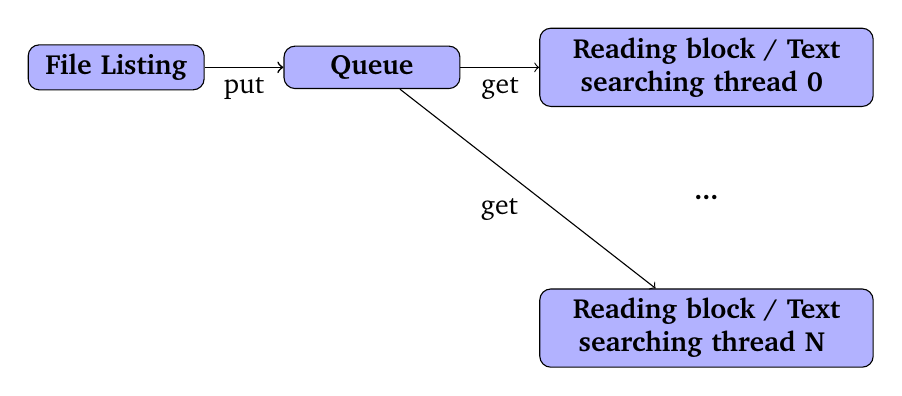
\begin{tikzpicture}[node distance=1cm]
    \node (FileListing) [rectangle, draw=black, rounded corners, fill=blue!30, text centered, anchor=north, text=black, text width=2cm] {
        \textbf{File Listing}
    };
    
    \node (Queue)  [] [rectangle, draw=black, rounded corners, fill=blue!30, text centered, anchor=north, text=black, text width=2cm, right=of FileListing] {
    	\textbf{Queue}
    }
    
    	edge[<-,bend angle=45,semithick] node[auto]{put} (FileListing);
    
   \node(FileProcessing0) [rectangle, draw=black, rounded corners, fill=blue!30, text centered, anchor=north, text=black, text width=4cm, right=of Queue] {
   	\textbf{Reading block / Text searching thread 0 }
   }
   	edge[<-,bend angle=45] node[auto]{get} (Queue);
   
   \node(Dots) [text centered, anchor=north, text=black, text width=4cm, below=of FileProcessing0] {
   	\textbf{...}
   };
   
   \node(FileProcessingN) [rectangle, draw=black, rounded corners, fill=blue!30, text centered, anchor=north, text=black, text width=4cm, below=of Dots] {
   	\textbf{Reading block / Text searching thread N }
   }
   	edge[<-,bend angle=45] node[auto]{get} (Queue);
\end{tikzpicture}

In application parameter you can specify the number of threads for file processing, it makes easy to setup single-thread environment (just set number of threads to 0). In order to determine what is the cost of searching algorithm I've implemented two different kind of text searching algorithm: naive search (complexity: $O(m + n)$) and Knuth-Morris-Pratt algorithm (complexity: $O(m) + O(n)$), where $m$ -- length of string pattern, $n$ -- length of searchable string.
 
\section*{Tests}

\subsection*{Environment}

\begin{verbatim}
Processor Name: Intel Core 2 Duo (1x2.66 GHz, 2 Cores, L2 Cache: 3Mb)
Memory: 4 GB (2x2Gb, DDR3, 1067 MHz, ECC: Disabled)
Bus Speed: 1.07 GHz
System Version: Mac OS X 10.6.8 (10K540), Kernel Version: Darwin 10.8.0

java version "1.6.0_26"
Java(TM) SE Runtime Environment (build 1.6.0_26-b03-384-10M3425)
Java HotSpot(TM) 64-Bit Server VM (build 20.1-b02-384, mixed mode)

VisualVM bundled with java is used to collect thread statistics.
\end{verbatim}

\subsection*{HDD}

Note: Before each start I'll flush operating system disk cache using command 'purge'.

\subsubsection*{Single-threaded approach}
Algorithm: Naive search and KMP search\\
Files to be processed: 11549\\
String pattern length: 4\\

First of all, let's do profiling to understand what is the most expensive step in our algorithm. Of course, file i/o operations on the first place (actually my hdd is very slow), look at $FileInputStream.read(byte[],int,int)$ -- 74.3\% of CPU time.

\begin{center}
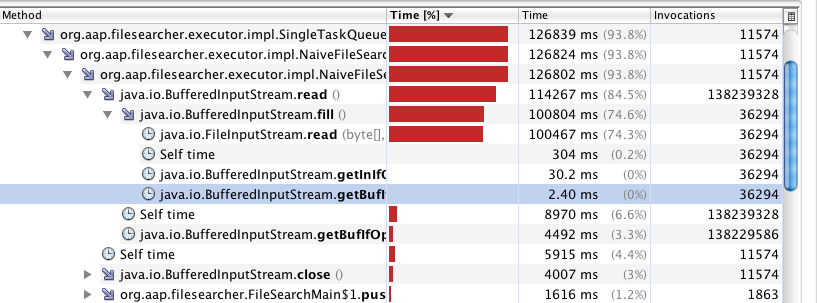
\includegraphics[width=16cm]{0Threads_Naive_11549_Profiling.png}
\end{center}

If we change implementation of the search algorithm with KMP (Knuth-Morris-Pratt) we got results more faster, $FileInputStream.read(byte[],int,int)$ now took about 83.8\% of CPU time (and total execution time less than for previous one for several seconds), that's means our application works more with i/o operations and it is good cause it is main bottleneck for our task. Also, KMP works much more better cause it doesn't use $BufferedInputStream$ $mark(int)$/$reset()$ mechanism (cause it is linear algorithm).

% string pattern length = 4
% buffer = 8192
% Execution time: 127796 msec (threads uptime: 0 msec), files processed: 11580
% Speed: 90 files per sec
% Execution time: 123652 msec (threads uptime: 0 msec), files processed: 11580
% Speed: 93 files per sec

% buffer = 65536
% Execution time: 113167 msec (threads uptime: 0 msec), files processed: 11580
% Speed: 102 files per sec
% Execution time: 105180 msec (threads uptime: 0 msec), files processed: 11580
% Speed: 110 files per sec

% string pattern length = 90
% Execution time: 118532 msec (threads uptime: 0 msec), files processed: 11580
% Speed: 97 files per sec
% Execution time: 109470 msec (threads uptime: 0 msec), files processed: 11580
% Speed: 105 files per sec

\begin{center}
\begin{tabular}{|c|c|c|c|}
\hline
Algorithm & Buffer &  Pattern length  & Time \\
\hline
\hline

Naive & 8192 & 4 & 127.796sec \\
\hline

KMP & 8192 & 4 & 123.652sec \\
\hline

Naive & 65536 & 4 & 113.167sec \\
\hline

KMP & 65536 & 4 & 105.180sec \\
\hline

Naive & 65536 & 90 & 118.532sec \\
\hline

KMP & 65536 & 90 & 109.470sec \\
\hline
\end{tabular}
\end{center}

\subsubsection*{Multi-threaded approach}
Algorithm: KMP search (I've decided to use only KMP cause Naive search is too slow)\\
Threads: 2\\
String pattern length: 4\\

According to profiling results for each thread file i/o operations took about 72.1\% and execution result time is decreased.
\begin{center}
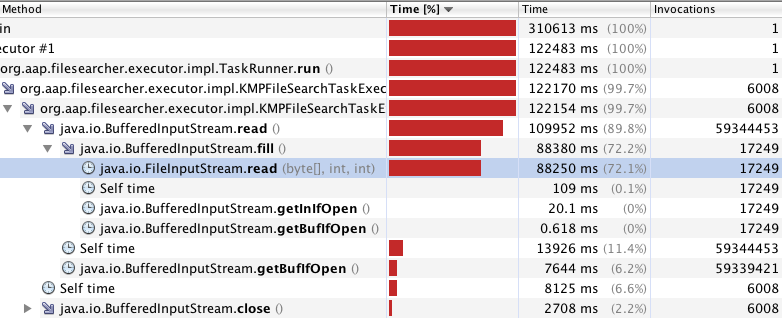
\includegraphics[width=16cm]{2Threads_KMP_11549_Profiling.png}
\end{center}

The result table of testing without profiling is placed below.
% buffer = 8192
% threads = 1
% Execution time: 104432 msec (threads uptime: 103961 msec), files processed: 11580
% Speed: 110 files per sec
% threads = 2
% Execution time: 101241 msec (threads uptime: 201356 msec), files processed: 11580
% Speed: 114 files per sec
% threads = 3
% Execution time: 95297 msec (threads uptime: 284565 msec), files processed: 11580
% Speed: 121 files per sec
% threads = 5
% Execution time: 92662 msec (threads uptime: 461146 msec), files processed: 11580
% Speed: 124 files per sec
% threads = 7
% Execution time: 83398 msec (threads uptime: 580616 msec), files processed: 11580
% Speed: 138 files per sec
% threads = 9
% Execution time: 92323 msec (threads uptime: 827370 msec), files processed: 11580
% Speed: 125 files per sec
% threads = 11
% Execution time: 115589 msec (threads uptime: 1266909 msec), files processed: 11580
% Speed: 100 files per sec

% buffer = 65536
% threads = 1
% Execution time: 116165 msec (threads uptime: 115718 msec), files processed: 11580
% Speed: 99 files per sec
% threads = 3
% Execution time: 102273 msec (threads uptime: 304343 msec), files processed: 11580
% Speed: 113 files per sec
% threads = 5
% Execution time: 100166 msec (threads uptime: 498622 msec), files processed: 11580
% Speed: 115 files per sec
% threads = 7
% Execution time: 102437 msec (threads uptime: 918008 msec), files processed: 11580
% Speed: 113 files per sec
% threads = 9
% Execution time: 101183 msec (threads uptime: 1106559 msec), files processed: 11580
% Speed: 114 files per sec
% threads = 13
% Execution time: 81896 msec (threads uptime: 1058536 msec), files processed: 11580
% Speed: 141 files per sec
% Execution time: 82723 msec (threads uptime: 1233897 msec), files processed: 11580
% Speed: 139 files per sec
% Execution time: 85794 msec (threads uptime: 1449396 msec), files processed: 11580
% Speed: 134 files per sec

\begin{center}
\begin{tabular}{|c|c|c|c|}
\hline
Buffer size & Threads count  & Time \\
\hline

8192 & 1 & 104.432 sec\\ \hline
8192 & 2 & 101.241 sec \\ \hline
8192 & 3 & 95.297 sec \\ \hline
8192 & 5 & 92.662 sec \\ \hline
8192 & 7 &  83.398 sec \\ \hline
8192 & 9 & 92.323 sec \\ \hline
8192 & 11 & 115.589 sec \\ \hline

65536 & 1 & 116.165 sec \\ \hline
65536 & 3 & 102.273 sec \\ \hline
65536 & 5 & 100.166 sec \\ \hline
65536 & 7 & 102.437 sec \\ \hline
65536 & 9 & 101.183 sec \\ \hline
65536 & 13 & 81.896 sec \\ \hline
65536 & 15 & 82.723 sec \\ \hline
65536 & 17 & 85.794 sec \\ \hline

\end{tabular}
\end{center}

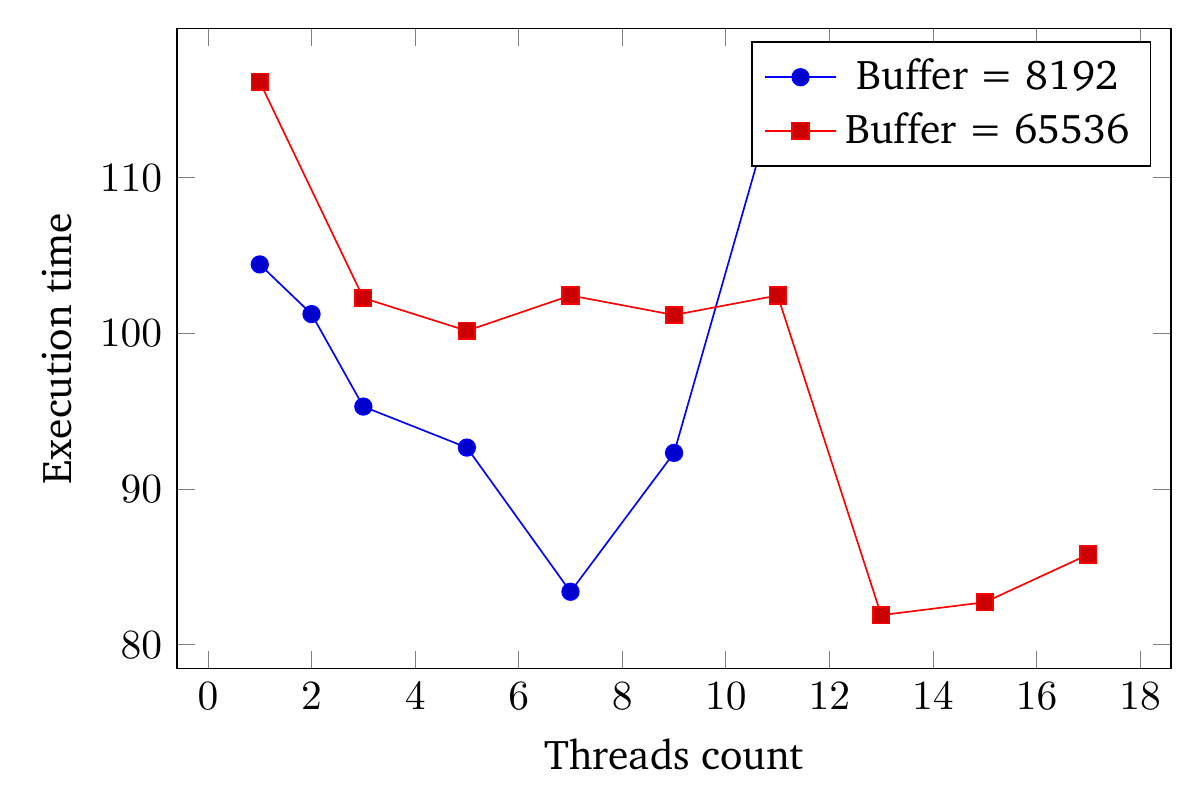
\begin{tikzpicture}[scale=1.5]
\begin{axis}[
xlabel=Threads count,
ylabel=Execution time,
height=7cm,
width=10cm ] 
\addlegendentry{Buffer = 8192}
\addplot coordinates {
( 1, 104.432 )
( 2, 101.241 )
( 3, 95.297 )
( 5, 92.662 )
( 7, 83.398 )
( 9, 92.323 )
( 11, 115.589 )};

\addlegendentry{Buffer = 65536}
\addplot coordinates {
( 1, 116.165 )
( 3, 102.273 )
( 5, 100.166 )
( 7, 102.437 )
( 9, 101.183 )
( 11, 102.437 )
( 13, 81.896 )
( 15, 82.723 )
( 17, 85.794 )};
\end{axis}
\end{tikzpicture}

% \subsection*{Memory drive}

% To reduce cost of the read operation I've decided to create memory drive and test application on memory drive.

\subsection*{Conclusion}
Even on regular HDD using multi-threaded approach I've got better results on some configurations. The results depends on count of threads and size of buffer which is used to read blocks from file. If we have a lot of threads we can see speed degradation cause our threads performs a lot of random access read operations. So, we need to select count of threads according to our resources. Optimal buffer size also can affect the results, cause sequential read in most cases faster than random read.

\subsection*{What's next?}
It is impossible to implement all ideas in short period of time, so, I think it is good to describe what I want to improve next:
\begin{itemize}
\item I think it is possible to get better results by putting i/o operations in separate thread pool. In this case, we can specify count of threads for i/o operations (it depends on controllers count) and we can specify count of thread for text pattern search procedure
\item BufferedInputStream is slow cause it is designed to be thread-safe and there is no way to maintain buffer manually (one worker requires only one buffer). It is possible to get better results using FileChannel API
\item It will be good to test application with memory disk. In this case, file i/o operations are really fast. It is interesting to know the results.
\end{itemize}

\newpage
\section*{Application options}

\begin{verbatim}
java FileSearcher [options] [--] <path> <string pattern>
    Options:
        -t <n>  	Set processing threads count to <n> (Default: 5)
        -b <n>  	Set file-input buffer to <n> (Default: 8192)
        -c <charset>  	Set character set to <charset> (Default: "US-ASCII")
        -s      	Print stasts after processing (Default: no)
        -w      	Wait for user input before start (Default: no)
        -n      	Use Naive search algorithm (Default: no)

    <path> - root path
    <string pattern> - string pattern for search
\end{verbatim}

\end {document}

























